
\section{Introducción}
Las imágenes satelitales son una de las fuentes de información más útiles para estudiar patrones espaciales a gran escala (estudios urbanos, ecológicos, etc). Estas imágenes se toman por dispositivos desde el espacio. Estos satélites pueden ser de diversos tipos y diseños, muchas veces incluyen varios sensores para captar información de diversas secciones del espectro electromagnético a distintos niveles de detalle.

\\

\begin{figure}[h!]
\begin{center}
\leavevmode
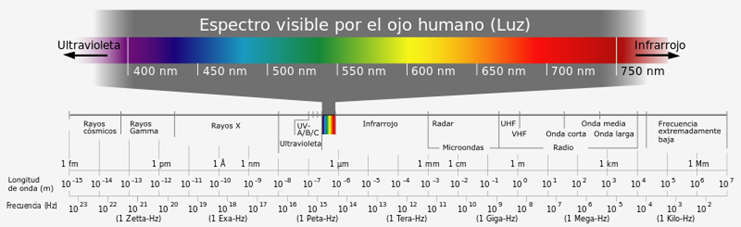
\includegraphics[width=5in]{1_espectro.png}
\end{center}
\caption{Espectro electromagnético}
\end{figure}

\\

 En este tutorial se explicará paso a paso cómo obtener imágenes de los satélites (Moderate-Resolution Imaging Spectroradiometer) MODIS y LANDSAT 8. Posteriormente cómo visualizarlas. El satélite MODIS capta información en 36 bandas del espectro electromagnético de 0.4 $\mu$m a 14.4 $\mu$m con resolución espacial (pixel) variante (2 bandas a 250m, 5 bandas a 500m y 29 bandas a 1km). El satélite Landsat 8 es el lanzamiento más reciente del programa Landsat. Capta información en 11 bandas del espectro, de 0.4 $\mu$m a 11.5 $\mu$m con una resolución espacial variante (8 bandas a 30m, 1 a 15m y 2 a 100m).

\newpage

Cada banda corresponde a un cierto "`color"' y más aún, a un cierto comportamiento físico determinado por cómo cierto terreno, y los objetos que allí se encuentran, reflejan la energía solar.

\\

\begin{figure}[h!]
\begin{center}
\leavevmode
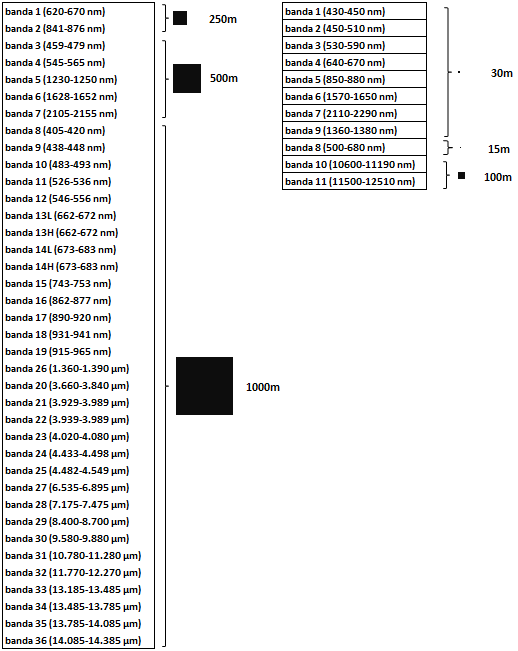
\includegraphics[width=4in]{2_bandas_modis_landsat.png}
\end{center}
\caption{Comparación bandas y tamaños de pixel: MODIS (izquierda) y Landsat 8 (derecha)}
\end{figure}

\newpage

\section{¿Por qué imágenes satelitales?}

Es importante recalcar que la utilidad de la información generada por estos satélites (imágenes) recae en que no sólo generan un modelo visual del lugar que están tomando, como lo hace una fotografía, si no que proveen de información física de los objetos que allí se encuentran. Distintos cuerpos, dependiendo de su naturaleza, reflejan la luz solar de distinta manera y en distintas intensidades.

\\
\begin{figure}[h!]
\begin{center}
\leavevmode
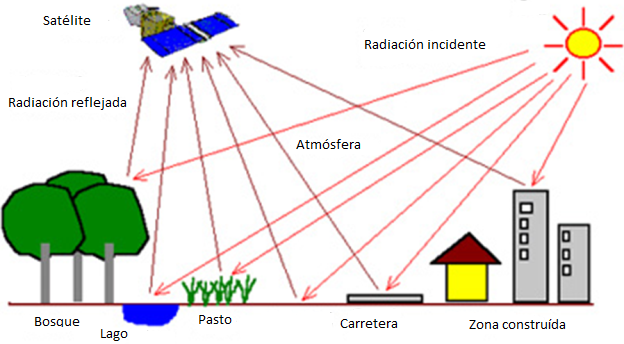
\includegraphics[width=4in]{3_sol_satelites.png}
\end{center}
\caption{Interacción: luz solar - atmósfera - terreno - atmósfera - satélite}
\end{figure}
\\

Por ejemplo es bien sabido que a muchas plantas las vemos verdes. Esto es resultado directo de que las hojas de estas plantas absorben más la parte de la luz solar que corresponde con el rojo y el azul puesto que utilizan esta energía en particular para llevar a cabo la fotosíntesis y alimentarse. Reflejan el verde por lo que lo que reciben nuestros ojos desde ellas nos hace visualizarlas en tonalidades de este color.


\\
\begin{figure}[h!]
\begin{center}
\leavevmode
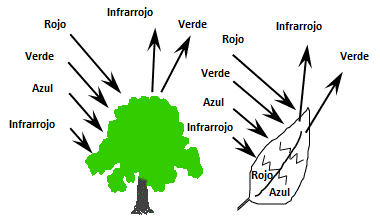
\includegraphics[width=3in]{4_plantas.png}
\end{center}
\caption{¿Por qué vemos verdes a las plantas?}
\end{figure}
\\

\newpage

De hecho, el concepto de "`color de un objeto"', por ejemplo una planta, es curioso.  Las plantas son del color del tipo luz que no abosorben, en este caso luz verde. Las plantas en realidad reflejan más la luz que correspondo al espectro infrarrojo, pero como se mostró en la figura 1.1, el ojo humano no es capaz de distinguir esta energía. Si pudiéramos ver "`en infrarrojo"' veríamos a las plantas infrarrojas. 




